\chapter{全文总结与展望}
\section{全文总结}
参考问题是头表脑电的主要缺陷之一,已有多数研究表明脑电频谱分析受到参考的影响。参考的不规范使用已成为定量脑电分析的首要问题。我们在第一部分(第二至四章)借助容积传导模型、等效偶极子理论、矩阵广义逆理论和贝叶斯统计学研究了影响参考选择的物理因素、参考选择的模型证据并推导出单极参考家族的共同属性和联系。因为定量脑电是基于频谱分析及谱特征的方法,与谱分析有关的技术也十分重要,我们在第二部分(第五至七章)依次研究谱质量控制准则、多国家脑电谱常模和谱成分分解与提取算法。图\ref{8:sum}是对全文结构的梳理,前后两部分是并列关系,但第一部分在内容上更加深
入全面,第二部分是对谱分析相关技术的初步探究。
\begin{figure}[!h]
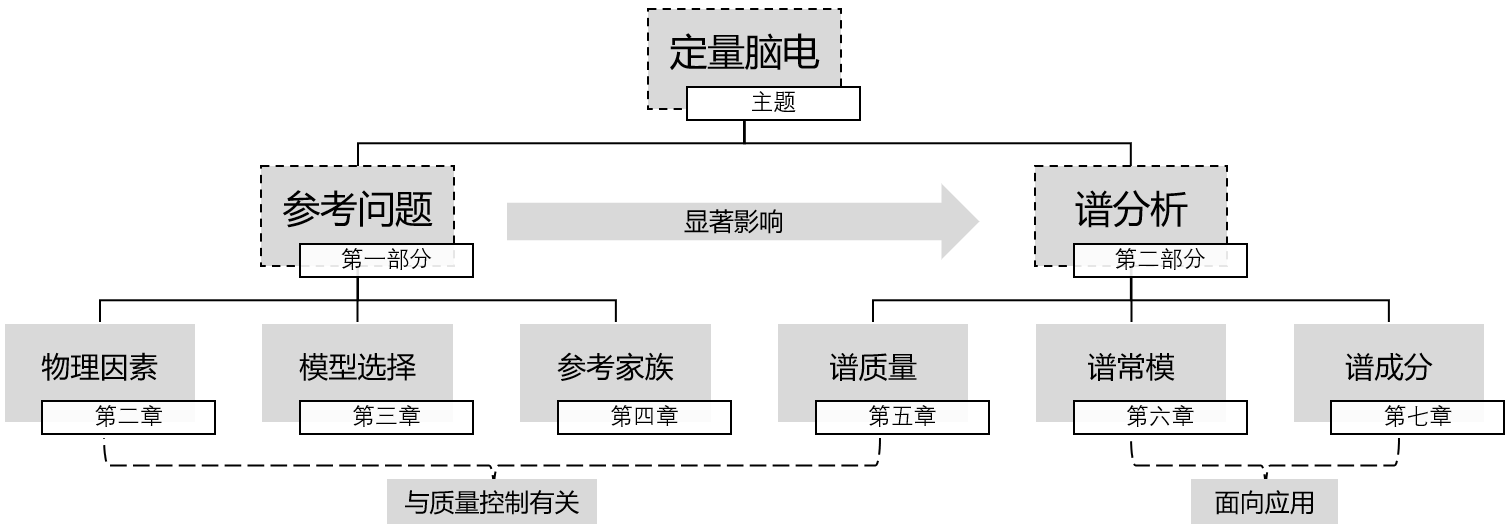
\includegraphics[width=\linewidth]{pic/sum/sum.png}
\caption{全文结构梳理。}
\label{8:sum}
\end{figure}

第一部分第二章中我们初步分析多种在线记录参考、平均参考和零参考的物理假设,从物理学的角度思考实际脑电数据采集中影响获取准确脑电电势、波形的因素,特别是参考选择和电极阵列配置等。我们仿真研究多种物理因素如何影响参考方法在变换脑电参考前后对逼近无穷远参考的效果。这些物理因素包括11种电极数、2种电极分布、电极噪声、头模型、神经源的位置方向等。出乎意料的是平均参考的效果并不随电极数增多而变优但依赖偶极子源活动方向和头表是否被电极宽泛覆盖,强调空间上尽可能广泛均匀采样而非电极的致密程度。零参考对多数因素表现出比平均参考更鲁棒的
性能,对头模型的扰动没有改变零参考的优势。这些新认识有助于我们在实际电极数和分布情况下选择最优参考。

第三章我们思考零参考与平均参考的区别,是否可能在数理统计学上找到二者性能差异的证据。我们首次提出脑电的广义线性参考模型,建立脑电无穷远参考估计的统一贝叶斯架构,得到估计理论无穷远参考脑电电位的通解。利用矩阵广义逆引理,我们发现平均参考和零参考都属于通解表达式,但分别是不同电极电位空间协方差先验下的特例。电极电位空间协方差独立同分布先验的结果是平均参考,而协方差中考虑容积传导效应的结果是零参考。将广义参考模型和通解变换到标准脊回归形式,我们使用广义交叉验证、Akaike、Bayesian等信息准则分析仿真脑电和89例实际脑电比较平均参考和零参考两种模型。仿真和实际数据一致说明零参考比平均参考模型更优,不同的协方差先验也给出二者区别的解释。参考的统一贝叶斯架构提供了零参考与平均参考模型区别的数理统计学证据。

第四章我们反思更多常见的脑电参考,分析多种单极参考的区别与联系。首先通过特殊矩阵逆引理证明零参考是一种单极参考;写出零参考和平均参考的物理约束表达式,从欠定的线性回归推导出零参考和平均参考,说明二者是不同物理假设下的合理估计量。最后,我们建立单极参考家族,找到所有单极参考间的联系,首次总结出无记忆性、满秩减一性、正交投影加权中心化属性,这些属性对实际数据分析中参考变换具有重要指导意义。至此,我们系统性地从偶极子、矩阵广义逆、贝叶斯统计学等角度分析了零参考、平均参考和其他单极参考的区别和联系,为实际中参考选择奠定坚实的理论基础。

第二部分第五章中我们首先描述多通道脑电谱曲线的同构问题使我们认识到脑电预处理可能存在问题。基于强力伪迹去除算法但无质量控制的预处理步骤可能会在去噪同时丢失脑活动有关信号,导致预处理完毕数据虽接近正常波形但频谱信息被破坏,严重影响定量脑电分析。若交叉谱或多通道功率谱同构则共同第一主成分绝对占优,我们基于共同主成分分析首次提出表征交叉谱同构异质的PaLOS准则。为验证PaLOS准则,我们分析电极配置、预处理不同的3个数据库共1525例脑电,然后研究PaLOS准则如何随预处理工具集成一体化平台-Automagic软件中主要步骤而变化。我们发现PaLOS准则与数据预处理程度有关,随预处理步骤变化,能有效表征谱的同构异质程度。有望在大样本频谱分析中使用PaLOS准则对预处理后的数据进行初筛。

第六章我们用古巴、美国、瑞士等三个国家535例覆盖生命周期的脑电数据,探究建立脑电谱常模的可能性。基于线性混合效应模型分析和模型比较,我们发现国家和个体这两种因素并不重要。通过分步模型选择和局部加权的非参数回归得到三个国家谱数据关于年龄和频率变化的脑电谱常模演化曲面,曲面中的低频$\delta$、$\theta$节律随年龄增长逐渐消失,高频$\alpha$节律随年龄增长逐渐增强并贯穿整个生命周期。该结果与以前基于单个国家或局部地区的研究结果一致,是首个建立多国家脑电谱常模的研究。这为将来建立独立于民族、文化的国际通用谱常模进行大尺度定量脑电研究提供了范例。

第七章中针对现有谱成分提取方法存在谱曲线拟合准则不具有统计学意义、参数拟合不能鲁棒地拟合形态各异谱成分的问题,我们首次提出基于Whittle似然准则和单调性约束的非参数拟合$\xi\pi$模型。我们在实际数据中得到比FOOOF模型更好的效果,应用$\xi\pi$模型到1772例颅内脑电数据进行谱成分分解和参数提取,得到符合物理解释的参数分布。基于高斯过程回归,我们用大脑中部分观测数据的谱成分参数估计任意频率全脑空间任意位置的谱值得到全脑空间的节律振荡谱地形图。这种全脑空间谱地形图可能作为溯源方法研究的一种参考标准或定量脑电分析源空间意义的谱常模。

整体上,第一部分按照物理因素、统计模型选择、矩阵广义逆理论下单极参考联系与属性逐渐递进的关系研究了参考选择问题,丰富了定量脑电参考研究的理论成果,这些成果已被国际人类脑影像研究组织出版的神经影像数据分析与共享最佳实践白皮书\citing{pernet2018best}收录,被R. A. Salido
-Ruiz等\citing{salido2019unified}的研究肯定,也正被EEGLAB\citing{delorme2004eeglab}、零参考软件\citing{dong_l_matlab_2017}等整合使用。第二部分依次研究谱质量控制提出筛选准则、建立多国家脑电数据谱常模、发展能鲁棒分解谱成分提取特征的$\xi\pi$模型并得到初步应用,
这些结果在BrainModes、OHBM等国际会议\citing{hu2018nonparametric,hu2020palos_o}上受到同行的积极评价。本文发展的参考新理论和谱分析新
技术对健全定量脑电分析方法、促进定量脑电的临床应用具有重要意义。

\section{后续工作展望}
本文仍存在以下不足,值得进一步研究:

第二章中,因为理论最优的无穷远参考脑电电位在实际数据中并不存在,我们只基于物理学假设进行了仿真比较。这种仿真中结果与实际数据采集和参考估计中的效果差异还不清楚。虽然实际中不可能获得理论最优的无穷远参考电位,我们可能通过设计实验范式,以特殊事件刺激下的诱发脑电特征或与认知活动密切相关的脑电波模式作为标准,验证不同的电极数目、分布等物理因素比较实际中参考的性能差异。考虑到参考可能对不同来源噪声的敏感度不同,我们希望能比较不同类型噪声时参考效果差异,分析复杂噪声源时的参考选择。

第三章中,理论分析认为传统零参考和平均参考都是理想无噪声假设下推导出的,我们提出正则化的具有去噪效果的零参考和平均参考。尽管仿真说明广义交叉验证是正则化参数选择的最优准则,还有待于在更多实际数据分析场景中进行验证。我们发现群体平均头模型可能具有和基于个体磁共振数据的头模型相似的效果,在实际中可以基于特定群体的磁共振数据估计建立模板头模型。

第四章中,我们认识到单极参考家族的共同属性。我们计划将这些属性编写到工具包中,提醒实际数据分析中注意应用这些属性。针对不当参考下的性能差异,我们可以制作详细的参考选择推荐表,规范电极数等因素下的合理参考选择。

第五章中,虽然我们提出的谱结构准则在数据库上得到验证,但目前只适于大样本脑电数据预处理后的初筛,还不能对脑电数据预处理程度和数据质量进行精准的表征。将来我们可能在分析大量数据预处理步骤和电生理专家辅助监督的基础上对筛选准则进行改进或提出其他的准则作为补充。

第六章中,我们初步研究肯定多国家间建立谱常模的可能性,但存在国家少、国家间样本量不匹配特别是部分国家年龄不均衡的问题。已有数据主要来自西方国家,我们将注意收集分析亚太地区的脑电数据使地域分布更均衡更代表国际化。未来,我们不仅希望国际同行积极合作建立开放共享的数据库构建更鲁棒的国际通用谱常模,还可能建立神经源空间的谱常模。

第七章中,虽然我们提出能进行谱分解和特征提取的$\xi\pi$模型,但只对单电极或某个源空间位置上的功率谱曲线分解和特征提取。如果考虑交叉谱并借助协方差统计学如黎曼学习,我们可能得到基于交叉谱或脑连接的谱常模空间流形,进而提取空间模式或者脑连接特征。这样有助于得到更细化的生物标记物,提高利用定量脑电进行分类识别诊断的准确率。

总体上我们还没有直接比较参考选择如何影响定量脑电谱分析。这是因为已有大量研究表明参考选择对频谱分析有影响,我们在第二部分中主要发展新算法改进定量脑电谱分析技术存在的不足。将来我们可以研究参考选择对定量脑电分析中每一步的影响,如探究零参考与平均参考对脑电谱常模估计和头表脑电谱成分参数的影响。本文第一部分研究的参考问题主要基于仿真分析,第二部分提出的谱分析新方法仅在部分数据上得到验证,脑电在实验室及医院的普及将允许我们在更多实例数据中验证并改进文中发展的新理论、新方法,使最终能应用于临床定量脑电分析。本文仅重点研究了参考和谱两方面,其他定量脑
电分析方法特别是头表微状态、源空间时变连接模式等时空动力学分析值得后续研究加以完善。